\documentclass[useAMS, usenatbib, preprint, 12pt]{aastex}
\usepackage{cite, natbib}
\usepackage{float}
\usepackage{epsfig}
\usepackage{cases}
\usepackage[section]{placeins}
\usepackage{graphicx, subfigure}
\usepackage{color}
\usepackage{bm}
\usepackage{enumerate}

\newcommand{\columbia}{1}
\newcommand{\oxford}{3}
\newcommand{\uw}{4}
\newcommand{\princeton}{2}
\newcommand{\naigrain}{333}
\newcommand{\nmcquillan}{100}
\newcommand{\nkois}{1102}
\newcommand{\nkoimcq}{275}
% \newcommand{\nkoigood}{222}
% \newcommand{\nkoibad}{49}
\newcommand{\kepexample}{1430163}
\newcommand{\kepexampleperiod}{4}
\newcommand{\aigrainexampleperiod}{20.8}
\newcommand{\Kepler}{{\it Kepler}}
\newcommand{\kepler}{\Kepler}
\newcommand{\corot}{{\it CoRoT}}
\newcommand{\Ktwo}{{\it K2}}
\newcommand{\ktwo}{\Ktwo}
\newcommand{\TESS}{{\it TESS}}
\newcommand{\LSST}{{\it LSST}}
\newcommand{\Wfirst}{{\it Wfirst}}
\newcommand{\SDSS}{{\it SDSS}}
\newcommand{\PLATO}{{\it PLATO}}
\newcommand{\Teff}{$T_{\mathrm{eff}}$}
\newcommand{\teff}{$T_{\mathrm{eff}}$}
\newcommand{\FeH}{[Fe/H]}
\newcommand{\feh}{[Fe/H]}
\newcommand{\ie}{{\it i.e.}}
\newcommand{\eg}{{\it e.g.}}
\newcommand{\logg}{log \emph{g}}
\newcommand{\dnu}{$\Delta \nu$}
\newcommand{\numax}{$\nu_{\mathrm{max}}$}
\newcommand{\acfRMS}{0.60}
\newcommand{\pgramRMS}{0.98}
\newcommand{\mcmcRMS}{0.46}

\begin{document}

\title{Inferring probabilistic stellar rotation periods using Gaussian
processes}

\author{%
   Ruth Angus\altaffilmark{\columbia},
   Timothy Morton\altaffilmark{\princeton}
   Suzanne Aigrain\altaffilmark{\oxford},
   Daniel Foreman-Mackey\altaffilmark{\uw}
   Suzanne Aigrain\altaffilmark{\oxford},
   \& Vinesh Rajpaul\altaffilmark{\oxford}
}

\altaffiltext{\columbia}{Simons Fellow, Department of Astronomy, Columbia
University, NY, NY, RuthAngus@gmail.com}
\altaffiltext{\oxford}{Subdepartment of Astrophysics, University of Oxford,
UK}
\altaffiltext{\uw}{Department of Astronomy, University of Washington, Seattle,
WA}
\altaffiltext{\princeton}{Department of Astrophysical Sciences, Princeton
University,  Princeton, NJ}

\begin{abstract}
The light curves of spotted, rotating stars are often non-sinusoidal and
quasi-periodic---spots are not static on the stellar surface and have finite
lifetimes causing stellar flux variations to slowly shift in phase.
A strictly periodic sinusoid is therefore not a representative model for the
light curve of star with a rotational signal.
Ideally, a physical model of the stellar surface would be conditioned on the
data, however the parameters of such models can be highly degenerate
\citep[\eg][]{Russell1906, Jeffers2009}.
Instead, we use an appropriate {\it effective} model: a Gaussian Process (GP)
with a quasi-periodic covariance kernel function.
By modelling the light curve with a GP, a highly flexible semi-parametric
function, we avoid the necessity of choosing a `best fitting' functional form,
whilst sampling directly from the posterior Probability Density Function (PDF)
of the periodic parameter and marginalising over the other kernel
hyperparameters.
We use \naigrain\ simulated light curves with a range of rotation periods to
    test the GP model and compare our results with a sine-fitting periodogram
    method and an AutoCorrelation Function (ACF) method.
The posterior PDFs of the parameters were sampled using the affine invariant
    ensemble Markov Chain Monte Carlo (MCMC) sampler {\tt emcee3}
    \citep{Foreman-Mackey2013}, and the GP operations were performed using the
    {\tt george} python package \citep{George}.
We demonstrate that rotation periods inferred via this method are more
    accurate than the periodogram and ACF methods.
Furthermore, the rotation periods are inferred probabilistically, allowing
    them to be easily incorporated into follow-on studies; inferring stellar
    ages or characterising star-planet interactions for example.
% Thehe ACF method is not applicable to unevenly spaced data,
% therefore it is inappropriate for the ~$10^7$ stellar light curves expected
% to be produced by \LSST\ unlike the GP method.
% Furthermore, the improvement is expected to be even more dramatic when applied
% to real, noisy {\it Kepler} light curves, since the GP method is well suited
% to modelling rotation signals and correlated noise simultaneously.

\end{abstract}

\section{Introduction}

The light curves of spotted, rotating stars are often non-sinusoidal and
Quasi-Periodic (QP).
These stars vary in brightness due to active regions on their surfaces which
rotate in and out of view.
The non-sinusoidal quality is caused by the complicated surface spot patterns
and the quasi-periodicity is produced both by the finite lifetimes of these
active regions and the presence of differential rotation on the stellar
surface.
A strictly periodic sinusoid is therefore not a good model for stellar light
curves.
In an ideal world, a physical model of the stellar surface would be
conditioned on the data.
A physically realistic model would perfectly capture the complexity of shapes
within stellar light curves as well as the quasi-periodic nature, allowing for
extremely precise probabilistic period recovery.
However, such physical models require many free parameters in order to
accurately represent a stellar surface and some of these parameters are
extremely degenerate \citep[\eg][]{Russell1906, Jeffers2009}.
In addition to global stellar parameters such as inclination and rotation
period, each spot or active region should have (at minimum) a longitude,
latitude, size, temperature and lifetime.
Considering that many stars have on the order of hundreds of spots, the number
of free parameters quickly becomes unwieldy, especially if the posterior PDFs
of these parameters are explored with MCMC.
Simplified spot models, such as the one described in \citet{Lanza2014} where
only two spots are modelled, have produced successful results, however these
simplified models sacrifice some precision due to lack of model flexibility.
Instead of using a physical model for stellar light curves, we choose to use
an {\it effective} model: one which captures the behaviour but is not
physically motivated, although the parameters of this model may be {\it
interpreted} as physical ones.
An ideal effective model for the light curve of a spotted, rotating star is
one with a small number of non-degenerate parameters that is flexible enough
to perfectly capture non-sinusoidal, QP behaviour.
These requirements are fulfilled by a Gaussian process (GP) model.

The standard methods used for measuring rotation periods include detecting
peaks in a Lomb-Scargle \citep{Lomb1976, Scargle1982} (LS) periodogram
\citep[e.g.][]{Reinhold2013}, Auto-Correlation Functions (ACFs)
\citep{Mcquillan2013} and wavelet transforms \citep{Garcia2014}.
The precision of the LS periodogram and wavelet methods are limited by the
suitability of the model choice.
A sinusoid is used in the case of the LS periodogram and the wavelet method
relies on a choice of mother wavelet that is assumed to describe the data over
a range of transpositions \citep[see, \eg][]{Carter2010}.
In contrast, the ACF method is much better suited to signals that are
non-sinusoidal.
In fact, it doesn't matter what shape the signal is: as long as it is
approximately periodic the ACF will display peaks located at the rotation
period.
A drawback of the ACF method however, is that it requires data to be
evenly-spaced\footnote{\citet{Edelson1988} describe a method for computing
ACFs for unevenly-spaced data.} which is not exactly the case with \Kepler\
light curves (although in many cases it can be approximated as uniformly
sampled) and not nearly the case for the future large-scale survey instrument,
\LSST.
An ACF is also an operation performed on the data, not a generative model of
the data and is therefore not inherently probabilistic.
For this reason it is very difficult to estimate the uncertainty on an ACF
rotation period measurement.
% Many rotation periods in the literature have been inferred by measuring the
% position of the first peak in an ACF, however this approach can be dangerous.
% The exponential decay in correlation can shift the peak position short-wards
% of its true value, leading to an underestimate of the period.
% We return to this point in section \textsection \ref{sec:discussion}.

The motivation for developing a GP-based method for rotation period inference
is, firstly to measure more accurate and precise rotation periods using a
better-suited generative model than a sinusoid for the reasons explained
above.
Secondly, in order to infer {\it probabilistic} periods, i.e. to estimate the
posterior PDF of the rotation period and thereby produce a realistic and
estimate of its uncertainty.
Thirdly, to allow for an additional correlated noise model to be included
during regression, the parameters of which could be marginalised over.
% And fourthly to provide some way of determining whether a periodic model is
% supported by the data over a purely stochastic one.

GPs are commonly used in the machine learning community and increasingly
in other scientific fields, for example biology and geophysics.
More recently, GPs have been used in the astronomy literature \citep[see
\eg][]{Gibson2012, Haywood2014, Haywood2015, Evans2015, Rajpaul2015,
Rajpaul2016, Aigrain2016}.
% FIXME: CITATIONS Gibson, Aigrain, Evans, Rajpaul, Waldman(?), Cosmology,
% geology, biology, Rasmussen & Williams, etc.
They are useful in regression problems involving any stochastic process,
specifically when the probability distribution for the process is a
multi-variate Gaussian.
If the probability of obtaining a data-set is a Gaussian in $N$ dimensions,
where $N$ is the number of data points, that data-set can be described as, and
with, a Gaussian process.
An in-depth introduction to Gaussian processes is provided by
\citet{Rasmussen2005}.

GP models parameterise the covariance between data points and a kernel
function provides the form of covariance matrix parameterisation.
For example, take the time-series in figure \ref{fig:GP_example}.
This is the \kepler\ light curve of KIC \kepexample, a relatively active star that
rotates once every $\sim$ 4 days.
The stochastic variability in this time-series is typical of \kepler\ FGK
stars.
Clearly, data points in this light curve are correlated.
Points that are close together in time are tightly correlated and those that
are widely separated in time are loosely correlated.
The way in which the covariance varies with the separation between data points
is modelled when using GP regression; it is not the data but the {\it
covariance structure} that is modelled.
This fact is what gives GPs their flexibility---they can model any time
series with a similar covariance structure.
In addition, a very simple function can usually capture the covariance
structure of a light curve, whereas a much more complicated one may be
required to model the time-series itself.
% The light curve of \Kepler-452 has been modelled with a GP in figure
% \ref{fig:GP_example}, shown in orange.
In figure \ref{fig:GP_example} the light curve of KIC \kepexample\ has been
modelled with a GP.
% Both provide adequate fits to the data, however only the periodic kernel
% function, `QP' is a useful model because it has a periodic parameter.
% I return to this point shortly.

A range of kernel functions could be used to describe stellar variability.
For example, the simplest and most commonly used kernel function, the `Squared
Exponential' (SE) produces an adequate fit to the KIC \kepexample\ light
curve.
The SE kernel function is defined as,
\begin{equation}
k_{i,j} = A \exp \left(-\frac{(x_i - x_j)^2}{2l^2} \right).
\end{equation}
\label{eq:SE}
Here $A$ is the amplitude of covariance, $l$ is the length scale of
exponential decay and $x_i-x_j$ is the separation between data points.
The SE kernel function has the advantage of being very simple---it has just
two parameters, a covariance amplitude and length scale: $A$ and $l$.
If $l$ is large two data points far apart in $x$ will be tightly correlated,
and if small they will be loosely correlated.
Another property of the SE kernel function is that it produces functions that
are infinitely differentiable.
It is therefore possible to model a data set and its derivatives
simultaneously.
% \citep[see \eg][]{Rajpaul2015}
The SE kernel function is not a good model of the covariance in stellar light
curves, nor a {\it useful} one for the problem of rotation period inference
because it does not capture periodic behaviour.
In order to infer rotation periods it is necessary to use a periodic kernel
function.
For this reason, we use the `Quasi-Periodic' kernel function.
The QP kernel function is defined as
\begin{equation}
k_{i,j} = A \exp \left(-\frac{(x_i - x_j)^2}{2l^2} -
\Gamma^2 \sin^2(\frac{2\pi}{P}) \right).
\end{equation}
\label{eq:QP}
It is the product of the SE kernel function, which describes the overall
covariance decay, and an exponentiated, squared, sinusoidal kernel function
that describes the periodic covariance structure.
$P$ can be interpreted as the rotation period of the star and $\Gamma$
controls the amplitude of the $\sin^2$ term.
If $\Gamma$ is very small, only points almost exactly one period away are
tightly correlated and points that are slightly more or less than one period
away are very loosely correlated.
If $\Gamma$ is large, points separated by one period are tightly
correlated and points separated by slightly more or less are still highly
correlated although less so.
This kernel function allows two data points that are separated in time by one
rotation period to be tightly correlated, while points separated by half a
period can be weakly correlated.
We also use an extra parameter, $\sigma$ which is an additional white noise
term added to the diagonal elements of the covariance matrix.
It is the fraction by which the observational uncertainties have been
underestimated --- if the uncertainties reported on the data are too small,
this parameter will be non-zero.
In practice however, this parameter should always be non-zero when performing
GP regression.
This is because the covariance matrix must be positive definite, however
matrix inversion performed using most solvers is approximate, not exact,
therefore slight deviations from positive definiteness can arise.
Including a small amount of extra variance in the model allows enough
flexibility that the matrix inversion algorithms do not run into numerical
issues.

This QP kernel function was used to produce the model shown in figure
~\ref{fig:GP_example}.

In order to infer a stellar rotation period from a light curve, we fit a GP
model with a QP kernel function to the data.
The likelihood of the model, conditioned on the data could then be maximised
in order to find the maximum likelihood value for $P$.
In this study however, the full posterior PDFs of the parameters are explored
using MCMC.
This approach comes at a cost: a GP model is expensive to compute once as it
requires an inversion and determinant evaluation of the covariance matrix, let
alone the many thousands of times that is necessary to fully explore the
posteriors of the parameters.
Fully exploring the posterior PDF of $P$ is important however, as it provides
an accurate estimate of the uncertainty on the rotation period.

\begin{figure}
\begin{center}
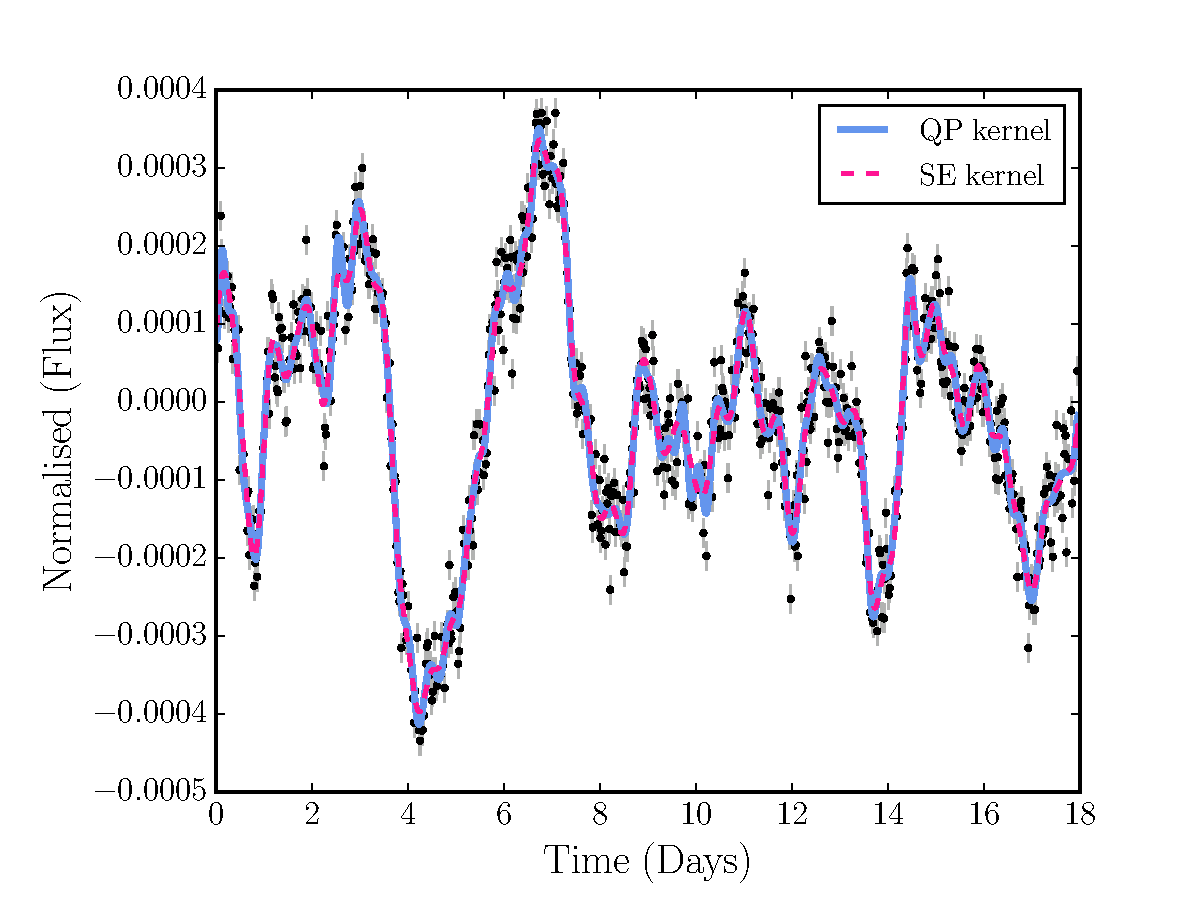
\includegraphics[width=6in, clip=true]{figures/001430163.pdf}
\caption[A light curve with a GP model.]
{Light curve of KIC \kepexample, an active star with a rotation period of
$\sim$ \kepexampleperiod\ days.
The blue line shows a fit to the data using a Gaussian process model with a QP
covariance kernel function.}
\label{fig:GP_example}
\end{center}
\end{figure}

In \textsection \ref{sec:simulations} of this paper we describe the simulated
light curves used to test rotation period inference methods.
In \textsection \ref{sec:method} we describe the various methods used to
recover the rotation periods: the periodogram, ACF and GP methods.
In \textsection \ref{sec:kepler} we apply our method to real \kepler\ data and
the results of the paper are discussed in \textsection \ref{sec:discussion}.

\section{Simulated light curves}
\label{sec:simulations}

In order to test the GP method we attempted to the measure rotation periods of
a set of simulated light curves.
We used \naigrain\ light curves generated for the \citet{Aigrain2015}
`hare and hounds' rotation period recovery experiment.
These light curves were simulated by placing dark, circular spots with slowly
evolving size, on the surface of bright, rotating spheres, ignoring
limb-darkening effects.
\citet{Aigrain2015} simulated one thousand light curves in order to test the
ability of participating teams to recover both the stellar rotation periods
and the rotational shear: the amplitude of surface differential rotation.
% Since we are not interested in recovering differential rotation we only used
% those light curves simulated {\it without} differential rotation, of which
% there are \naigraincurves.
For the purpose of demonstrating that our method can recover rotation periods,
we selected only the \naigrain\ out of the 1000 without differential
rotation.
We opted to use only solid-body rotators because differential rotation may
produce some additional scatter in the rotation period measurements recovered.
In future we intend to test whether we can recover differential rotation using
the GP method and will then use the full set of 1000 light curves.
The distributions of input parameters used to generate these light curves are
listed in \citet{Aigrain2015}.
Light curves were simulated with a real \Kepler\ long-cadence time array:
one data point every thirty minutes over a four year duration.
90\% of the rotation periods of the simulations were randomly drawn from a
log-uniform distribution between 10 and 50 days and 10\% from a log-uniform
distribution between 1 and 10 days.
A histogram of the \naigrain\ solid-body rotation periods is shown in figure
\ref{fig:period_hist}.
The light curves were also generated with a range of stellar inclination
angles, activity levels, spot lifetimes and more.
Once simulated, the light curves were added to real \kepler\ light curves with
no obvious astrophysical variability in order to preserve the noise properties
of the time series.
Figure \ref{fig:demo_lc} shows an example of a simulated light curve with a
period of \aigrainexampleperiod days.

The ranges and distributions of the physical stellar parameters used in the
simulated light curves are tabulated below, in table
\ref{tab:simulation_parameters}, and figure \ref{fig:period_hist} shows the
distribution of rotation periods in the \citet{Aigrain2015} sample.

\begin{table*}
\begin{center}
\caption{Ranges and distributions of parameters used to simulate light curves
in \citet{Aigrain2015}}
\begin{tabular}{lcc}
\hline\hline
    Parameter & Range & Distribution \\
    \hline
    Rotation period, $P_{rot}$ & 10 - 50 days (90\%) & log uniform \\
    & 1 - 10 days (10\%) & log uniform \\
    Activity cycle length & 1 - 10 years & log uniform \\
    Inclination & 0 - 90$^\circ$ & Uniform in $\sin^2i$ \\
    Decay timescale & (1 - 10) $\times P_{rot}$ & log uniform \\
\hline
\end{tabular}
\end{center}
\end{table*}
\label{tab:simulation_parameters}

\begin{figure}
\begin{center}
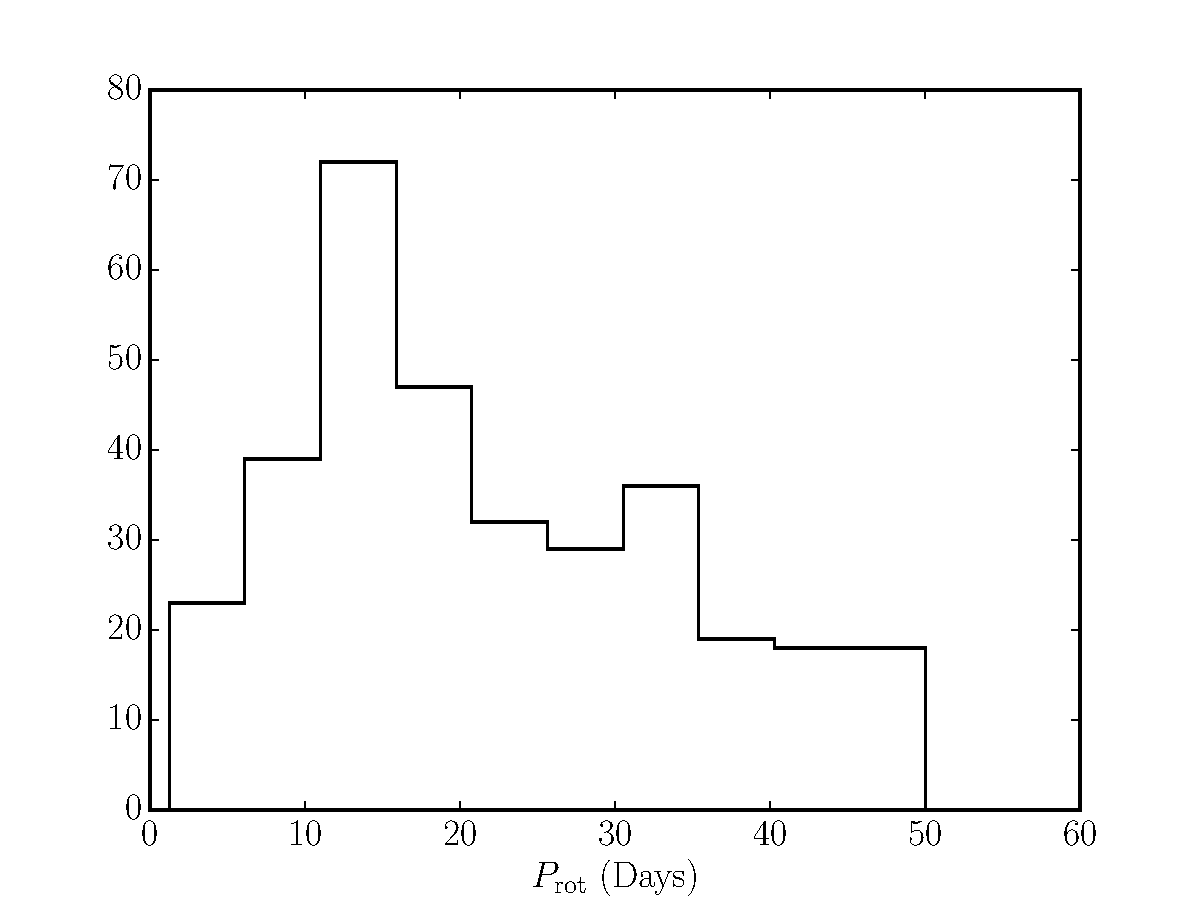
\includegraphics[width=6in, clip=true]{figures/period_hist.pdf}
\caption{A histogram of the rotation periods used to generate the \naigrain\
simulated light curves in \citet{Aigrain2015}.}
\label{fig:period_hist}
\end{center}
\end{figure}

\begin{figure}
\begin{center}
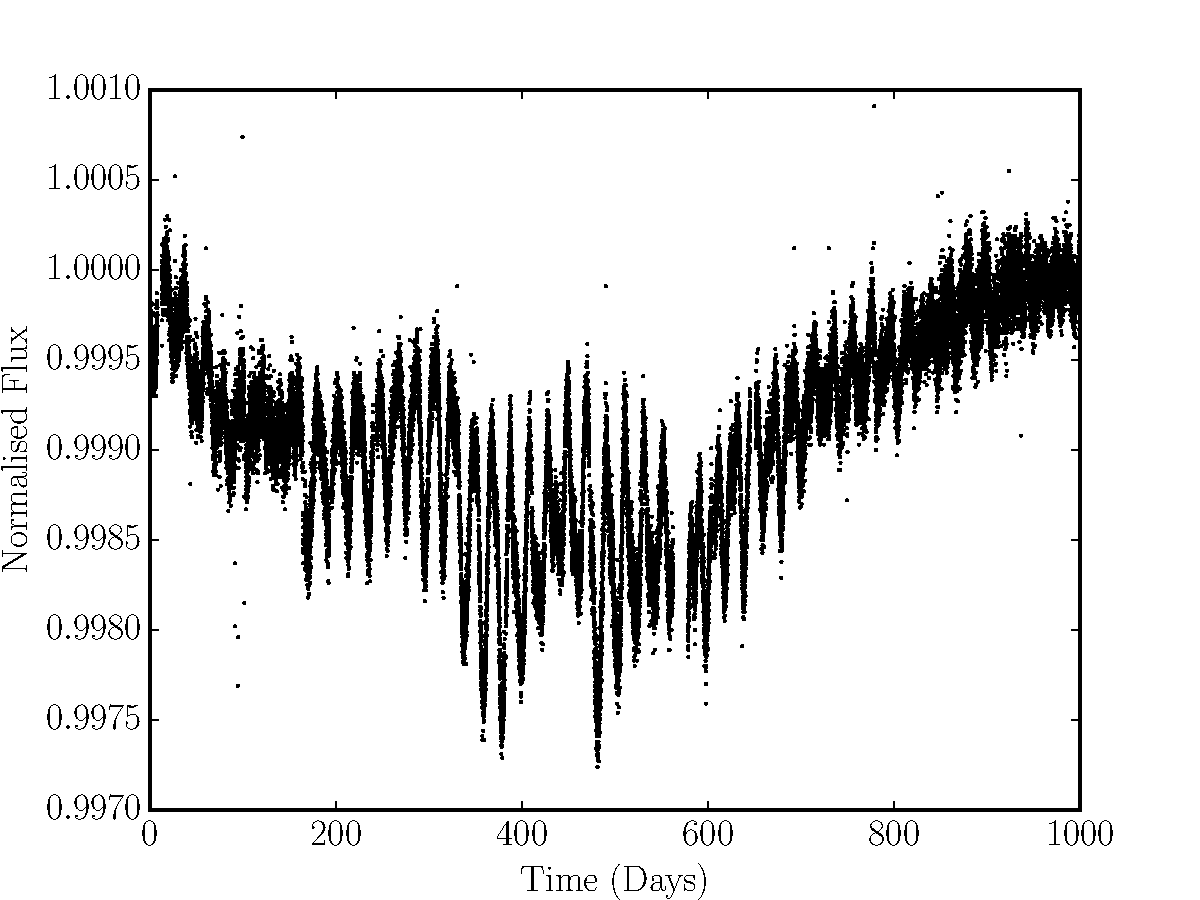
\includegraphics[width=6in, clip=true]{figures/demo_lc.pdf}
\caption[A simulated light curve.]
{An example simulated light curve. This `star' has a rotation period of
\aigrainexampleperiod\ days.}
\label{fig:demo_lc}
\end{center}
\end{figure}

% We attempted to recover the rotation periods of these \naigrain\ light curves
% using three methods: the ACF method; the LS periodogram method; and the GP
% method, and compared their performances.

\section{Rotation period recovery}
\label{sec:method}
\subsection{ACF}

We measured an ACF-based period for each light curve following the method of
\citet{Mcquillan2013}.
An ACF is calculated for each light curve and smoothed by convolving with a
Gaussian with $\sigma=9$ days.
A rotation period is estimated as the lag-time of the highest peak in the ACF,
less than 100 days.
This is not always the first peak: the second can be larger than the first if
there are two active regions at or near opposite longitudes on the surface of
the star---producing a light curve with two dips per rotation period.
We restrict our search to periods less than 100 days because this is the
maximum period that is realistically recoverable in \kepler\ light curves ---
instrumental noise significantly distorts signals on longer timescales.
An example ACF of the light curve in figure~\ref{fig:demo_lc} is shown
in figure \ref{fig:demo_acf}.

\begin{figure}
\begin{center}
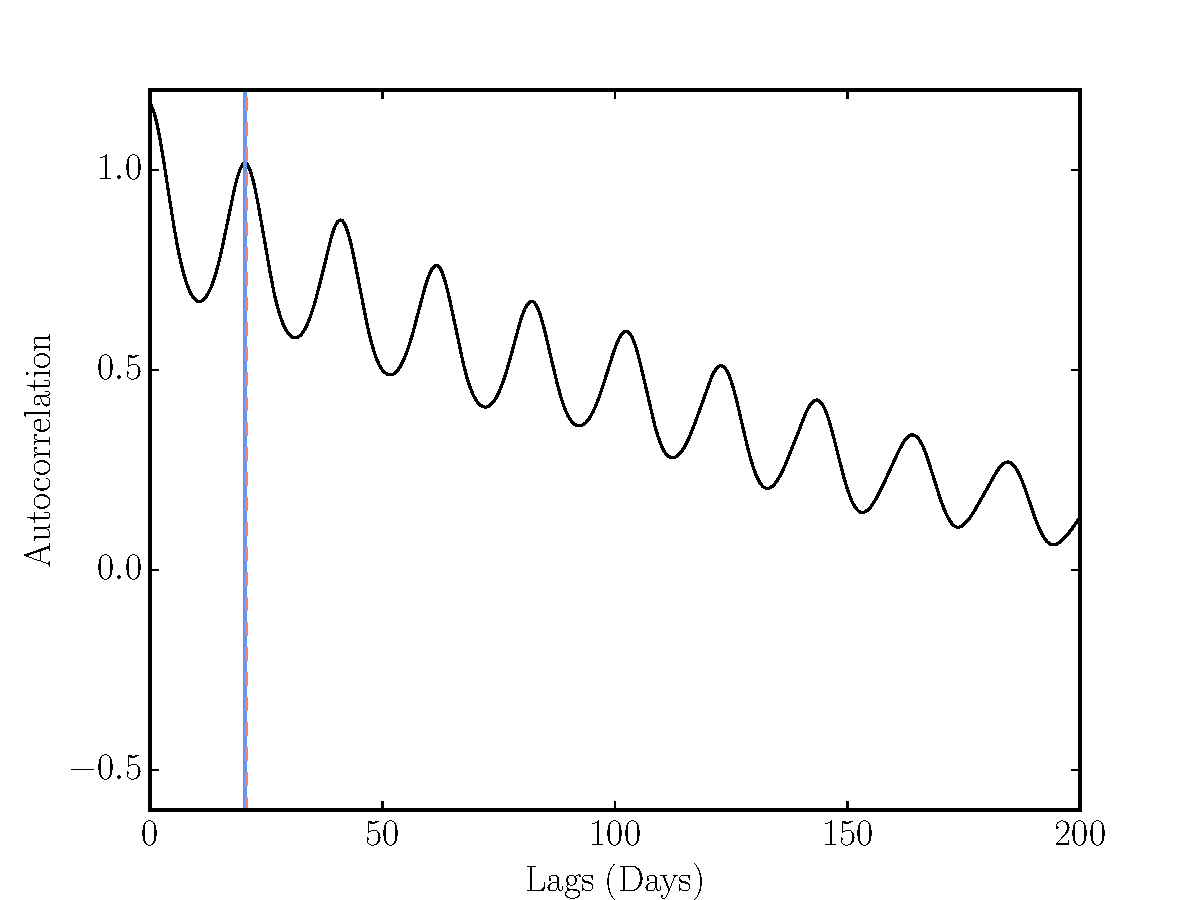
\includegraphics[width=6in, clip=true]{figures/demo_ACF.pdf}
\caption[ACF of a simulated light curve.]
{An autocorrelation function of the simulated light curve shown in figure
\ref{fig:demo_lc}.
The vertical blue line shows the period measured using the ACF method (20.4
days) and the pink dashed line shows the period that was used to simulate the
light curve (\aigrainexampleperiod\ days).}
\label{fig:demo_acf}
\end{center}
\end{figure}

The ACF method has proven to be extremely useful for measuring rotation
periods.
The catalogue of rotation periods of \Kepler\ stars provided in
\citet{Mcquillan2013} has been widely used by the community and has provided
ground-breaking results for stellar and exoplanetary science.
The results of the ACF method as tested in \citet{Aigrain2015} were positive
(see, for example their figure 8) as it produced a large number of accurate
rotation period measurements.
Another advantage of the ACF method is that it is fast to implement.
A clear disadvantage however, as already mentioned above, are the poorly
defined uncertainties for rotation periods estimated using an autocorrelation
function.
This is related to the fact that ACF period detection is a non-probabilistic
method, another drawback of ACF periods.

We applied the ACF method to the sample of \naigrain\ simulated light
curves.
Periods measured using the ACF method are plotted against the original
rotation period values used to generate the light curves in figure
\ref{fig:compare_acf}.
The $2n$ and $\frac{1}{2}n$ harmonic lines are shown as dashed lines.
The Median Absolute Deviation (MAD) of the ACF-recovered periods is \acfRMS\
in log-space (1.8 days).
The agreement between the injected and recovered rotation periods is good in
general, however some rotation periods are drastically over- and
underestimated.
Of the points clustered close to the $x=y$ line, more fall slightly below it
than above it, \ie\ rotation periods are preferentially underestimated.
This is a feature of the peak position measurement method that is performed on
the ACF.
ACFs of stellar light curves have similar functional forms to the QP kernel
function in equation \ref{eq:QP}: periodic functions added to decaying
exponentials.
In such functions the peak positions can be shifted towards the left, the
short period end, because the decaying exponential raises the left side of
each peak more than the right.
It is possible to model this effect, however the standard practice is to
simply measure the peak position without taking it into account.
We adopt the standard practice approach here in order to provide a comparison
between our new method and that used largely in the literature.

\begin{figure*}
\begin{center}
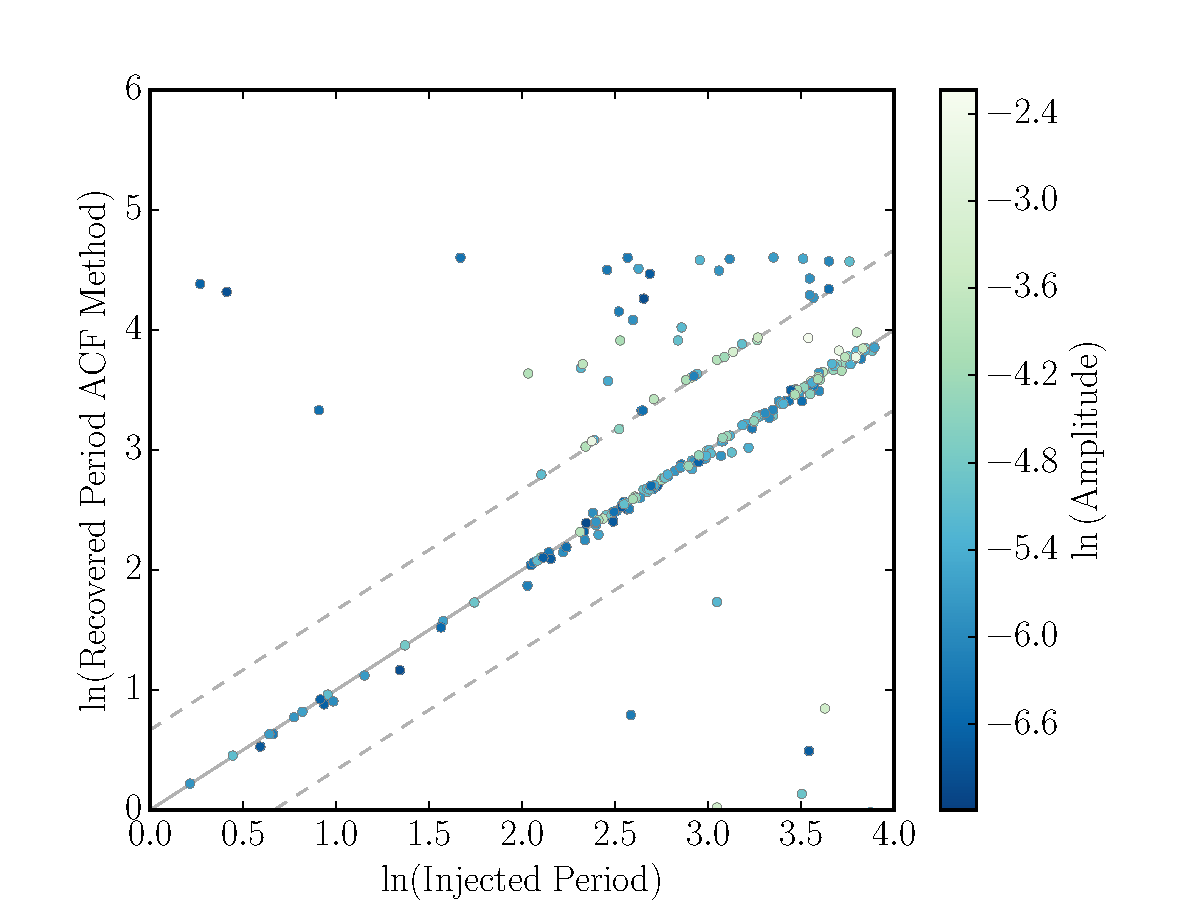
\includegraphics[width=6in, clip=true]{figures/compare_acf.pdf}
\caption[ACF results.]
{The `true' rotation periods used to generate \naigrain\ simulated light
curves vs the rotation periods measured using the ACF technique.
    Several light curves have over-estimated rotation periods and some
    are drastically underestimated.}
\label{fig:compare_acf}
\end{center}
\end{figure*}

\subsection{LS periodogram}

For each simulated light curve, a LS periodogram
\footnote{LS periodograms were calculated using the gatspy Python module:
\url{https://github.com/astroML/gatspy/tree/master/gatspy/periodic}.}
was computed over a grid of 10,000 periods, evenly spaced in frequency,
between 1 and 100 days.
The period of the highest peak in the periodogram was adopted as the rotation
period.
The resulting recovered rotation periods are plotted as a function of the true
periods in figure \ref{fig:pgram_compare}.
The MAD for rotation periods measured using the LS periodogram technique is
\pgramRMS\ in log-space (2.7 days).
There is a large number of drastically overestimated periods recovered using
the periodogram.
Excess power at long periods can be generated by long-term trends that are not
related to rotation.
This problem becomes exacerbated when instrumental noise is also present in
light curves.

\begin{figure*}
\begin{center}
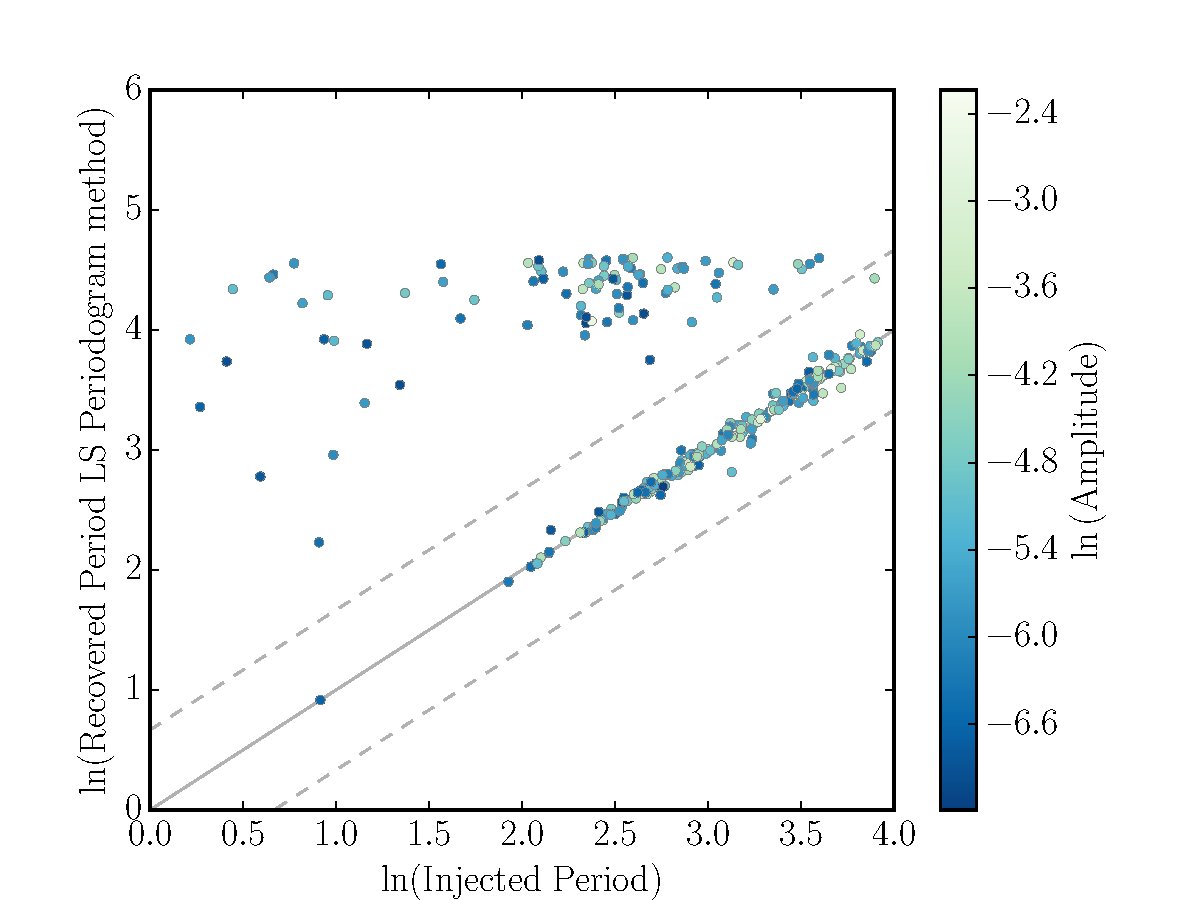
\includegraphics[width=6in, clip=true]{figures/compare_pgram.pdf}
\caption[LS periodogram results.]
{The `true' rotation periods used to generate \naigrain\ simulated light
curves vs the rotation periods measured using a LS periodogram technique.
In many cases a large peak at a long period was present in the periodogram,
    producing a significant over-estimate of the period.
    }
\label{fig:pgram_compare}
\end{center}
\end{figure*}

\subsection{The GP method}

In order to recover the rotation period of a simulated light curve using
Gaussian processes, we sample the following posterior PDF:
\begin{equation}
p({\bm \theta}\,|\,y) \propto \mathcal L(y\,|\,{\bm \theta}) p({\bm \theta}),
\end{equation}
\label{eq:posterior}
where $y$ are the light curve data, $\bm \theta$ are the hyperparameters
of the kernel described in equation \ref{eq:QP}, $\mathcal L$ is the
GP likelihood function, and $p({\bm \theta})$ is the prior on the
hyperparameters.  The GP likelihood is similar to the simple Gaussian likelihood
function used for optimisation problems where the uncertainties are
Gaussian and uncorrelated. The latter can be written
\begin{equation}
\ln \mathcal{L} = -\frac{1}{2}\sum_{n=1}^N\frac{(y_n-\mu)^2}{\sigma_n^2}
    - \frac{N}{2}\ln(2\pi\sigma_n^2),
\end{equation}
\label{eq:chi2}
where $y_n$ are the data, $\mu$ is the mean model and $\sigma_n$ are the
Gaussian uncertainites on the data.
The equivalent equation in matrix notation is
\begin{equation}
\ln \mathcal{L} = -\frac{1}{2}\bf{r}^T\bf{C}^{-1}\bf{r}-\ln|\bf{C}|
    + \mathrm{constant},
\end{equation}
\label{eq:lhf1}
where $\bf{r}$ is the vector of residuals and $\bf{C}$ is the covariance
matrix,
\begin{eqnarray}
	\mathbf{C} &=& \left (\begin{array}{cccc}
	\sigma^2_1 & \sigma_{2, 1} & \cdots & \sigma_{N, 1} \\
	\sigma_{1, 2} & \sigma^2_2 & \cdots & \sigma_{N, 2} \\
    && \vdots & \\
	\sigma_{1, N} & \sigma_{2, N} & \cdots & \sigma^2_N
\end{array}\right )
\end{eqnarray}
In the case where the uncertainties are uncorrelated, the noise is `white',
(which is a frequent assumption made by astronomers and is sometimes
justified) and the off-diagonal elements of the covariance matrix are zero.
However, in the case where there is evidence for correlated
`noise'\footnote{In our case the `noise' is actually the model!  Incidentally, this approach is the reverse of the regression techniques
usually employed by astronomers.
In most problems in astronomy one tries to infer the parameters that describe
the mean model and, if correlated noise is present, to marginalise over that
noise.
Here, the parameters describing the correlated noise are what we are
interested in and our mean model is simply a straight line at $y=0$.}, as in the
case of \Kepler\ light curves, those off-diagonal elements are non-zero.
With GP regression, a covariance matrix generated by the kernel function,
${\bf K}$ replaces ${\bf C}$ in the above equation.

Sampling the posterior PDF described above presents several challenges:
\begin{itemize}
\item Evaluating $\mathcal L$ for an entire \Kepler\ lightcurve
($\sim$40,000 points) takes about $\sim$5\,s--- too computationally expensive
to perform inference on large numbers of light curves\footnote{All
computational times cited in this section are based on evaluations on a
single core of a 2015 Macbook Pro, 3.1 GHz Intel Core i7.}.
The matrix operations necessary to evaluate the GP likelihood\footnote{These
operations use the fast matrix solver HODLR \citep{Ambikasaran2014},
implemented in the {\tt george} \citep{George} python package.} scale as
$N\ln(N)^2$, where $N$ is the number of data points in the light curve.

\item The flexibility of this GP model allows for posterior multimodality and
``over-fitting''--like behavior.
For example, if $l$ is small,  the non-periodic factor in the covariance
        kernel may dominate, allowing for a good fit to the data without
        requiring any periodic covariance structure---even if clear periodic
        structure is present.
Additionally, if $\Gamma$ is too large, the GP model becomes extremely
        flexible and can fit the data without varying the period.

\item In some cases, the posterior may also be multi-modal in period---that is,
there may be significant posterior density at half or twice the true period $P$.
\end{itemize}

We address the difficulty of computational speed in two distinct ways:
subsampling the data and splitting the light curve into independent sections.
To subsample, we randomly select 1/30th of the points in the full light curve
(an average of $\sim$1.5 points per day).
This decreases the likelihood evaluation time by a factor of about 50, down to
about 100\,ms.
We then split the light curve into equal-sized chunks containing approximately
300 points per section (corresponding to about 200 days), and evaluate the
log-likelihood as the sum of the log-likelihoods of the individual sections
(all using the same parameters ${\bm \theta}$).
This reduces computation time because the section-based likelihood evaluation
scales as $mn\ln(n)^2$, where $n$ is the number of data points per section and
$m$ is the number of sections.
This method further reduces computation time for a typical light curve
(subsampled by a factor of 30) by about a factor of two, to about 50\,ms.

In order to manage the flexibilty of the GP model and focus on reliably
retrieving the period parameter, we also impose priors on the non-period GP
parameters, learned during the development of this method.
Beginning with very broad priors (uniform in log space between -20 and 20) on
all the parameters, we first explored the typical values of the non-period
parameters when the injected periods were successfully recovered.
We also experimented with constraining the allowed ranges of the parameters
after discovering that some regions of parameter space (such as large values
of $A$ and $\Gamma$ and small values of $l$) tended to allow fits that ignored
the desired periodicity.
The priors and bounds we used for this work are listed in table
\ref{tab:priors}.
We note that we do not have any specific quantitative justification for the
use of these priors, except that they produce good results for this particular
test set of light curves.
We thus caution that other data sets might have different noise properties,
potentially requiring modifications to these priors on the non-period
parameters (e.g., see Section \ref{sec:kepler}).
For the period prior, we tried two different methods: an uninformed (log-flat)
prior between 0.5\,d and 100\,d, and an ACF-informed prior (details in
Appendix).
% We note that our default prior for period is log-uniform between the bounds,
% but that we were also able to further improve our results by using an
% ACF-inspired prior.

To sample the posterior in a way that is sensitive to potential multimodality,
we use the \texttt{emcee3} MCMC sampler.
We initialize 500 walkers with random samples from the prior and use a mix of
different proposal distributions: specifically, a 2:2:1 mix of KDE,
differential evolution, and DESnooker moves.
[DFM: more words/citations here?]
We run fifty steps of the sampler at a time, checking for convergence after
each iteration, up to a maximum of fifty iterations.
We declare convergence if the total effective chain length is at least
8$\times$ the maximum autocorrelation time.
When convergence is achieved, we drop the first two autocorrelation lengths in
the chain as a burn-in, and randomly choose 5000 samples as representative of
the posterior.
This fitting process takes several hours for a typical simulated light curve,
though in some cases it can take 12 hours or longer to converge.

\begin{table*}
\begin{center}
\caption{Priors and bounds on the natural logarithms of the GP model
    parameters.}
\begin{tabular}{lcc}
Parameter & Prior & Bounds\\
    \hline
    $\ln A$ & $\mathcal N(-13, 5.7)$ & (-20, 0) \\
    $\ln l$ & $\mathcal N(7.2, 1.2)$ & (2, 20) \\
    $\ln \Gamma$ & $\mathcal N(-2.3, 1.4)$ & (-10, 3) \\
    $\ln \sigma$ & $\mathcal N(-17, 5)$ & (-20, 0) \\
    $\ln P $ & Uniform / ACF-based & ($\ln 0.5, \ln 100$) \\
\end{tabular}
\end{center}
\end{table*}
\label{tab:priors}

\begin{figure*}
\begin{center}
% 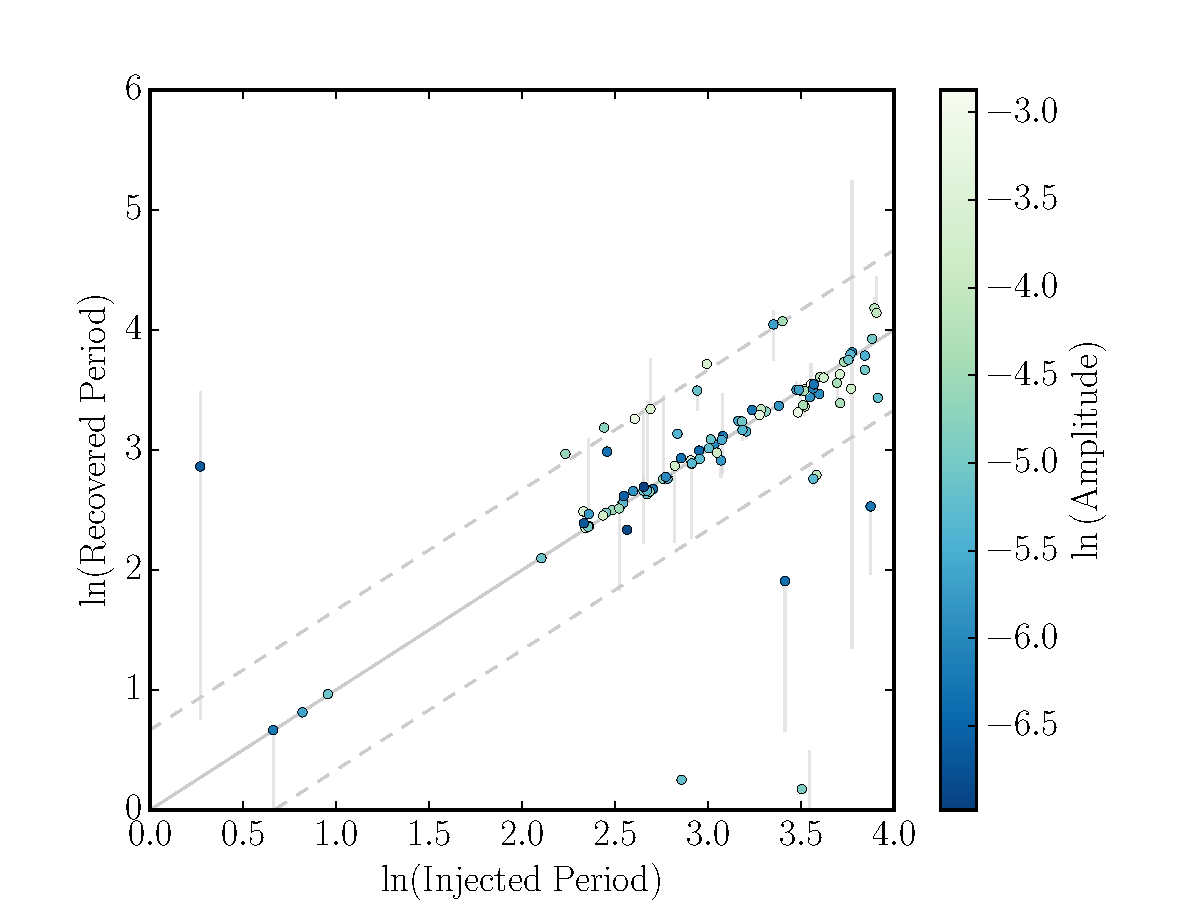
\includegraphics[width=6in, clip=true]{figures/compare_mcmc.pdf}
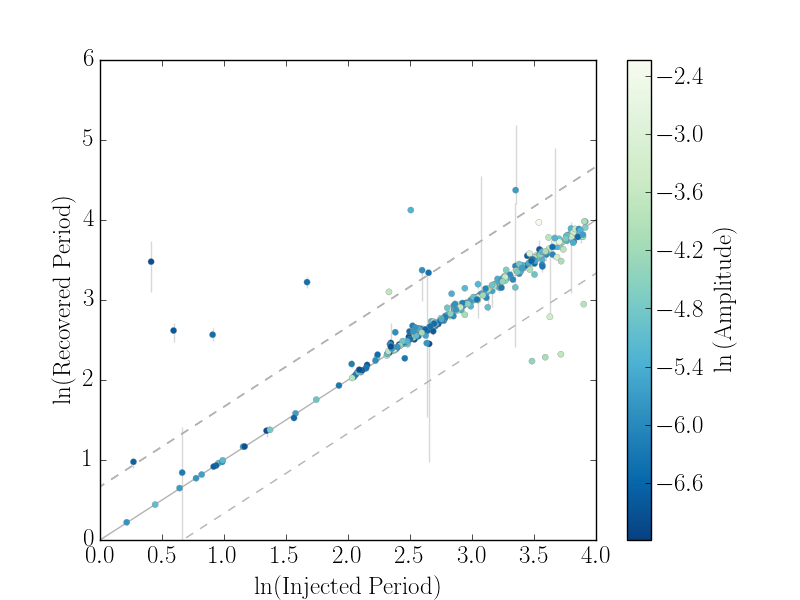
\includegraphics[width=6in, clip=true]{figures/comparison_emcee3_24_0.png}
\caption{The `true' rotation periods used to generate \naigrain\
simulated light curves vs the rotation periods measured using the GP
technique.
Since the posterior PDFs of rotation periods are often non-Gaussian,
the points plotted here are the highest likelihood samples.
The uncertainties are the 16th and 84th percentiles.
In many cases, the uncertainties are under-estimated.
The ACF-informed prior on rotation period used to generate these results is
    described in the appendix.
The MAD of these results is 0.38 in log-space, \ie\ 1.46 days.
    }
\label{fig:compare_mcmc_acfprior}
\end{center}
\end{figure*}

\begin{figure*}
\begin{center}
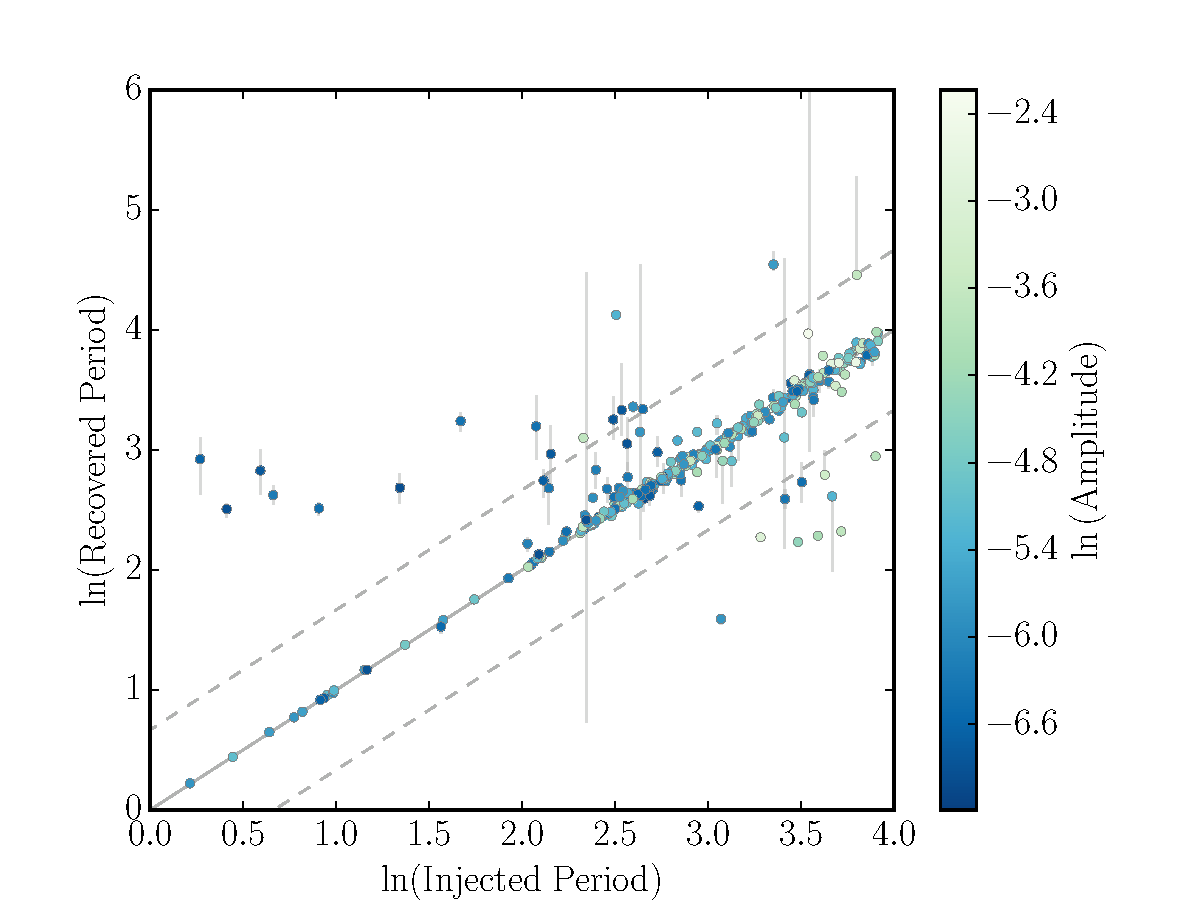
\includegraphics[width=6in, clip=true]{figures/comparison_noprior.pdf}
\caption{The `true' rotation periods used to generate \naigrain\
simulated light curves vs the rotation periods measured using the GP
technique with no .
Since the posterior PDFs of rotation periods are often non-Gaussian,
the points plotted here are the highest likelihood samples.
The uncertainties are the 16th and 84th percentiles.
In many cases, the uncertainties are under-estimated.
An uninformative prior, flat in the natural log of the rotation period between
    0.5 and 100 days was used to generate these results.
The MAD of these results is 0.48 in log-space, \ie\ 1.61 days.
    }
\label{fig:compare_mcmc_noprior}
\end{center}
\end{figure*}

Figures \ref{fig:compare_mcmc_acfprior} and \ref{fig:compare_mcmc_noprior}
summarize the results of this MCMC fitting procedure compared to the injected
`true' stellar rotation periods, for the uninformed and ACF-informed priors on
period, respectively.
Both the informative and uninformative prior versions of the GP method perform
better than the ACF and periodogram methods, with respective MADs of 0.38 and
0.48, compared to \acfRMS\ (ACF) and \pgramRMS\ (periodogram).
The marginal posterior distributions of the QP kernel hyperparameters for the
example simulated light curve in figure \ref{fig:demo_lc}, are shown in
figure \ref{fig:gp_posteriors}.

\begin{figure*}
\begin{center}
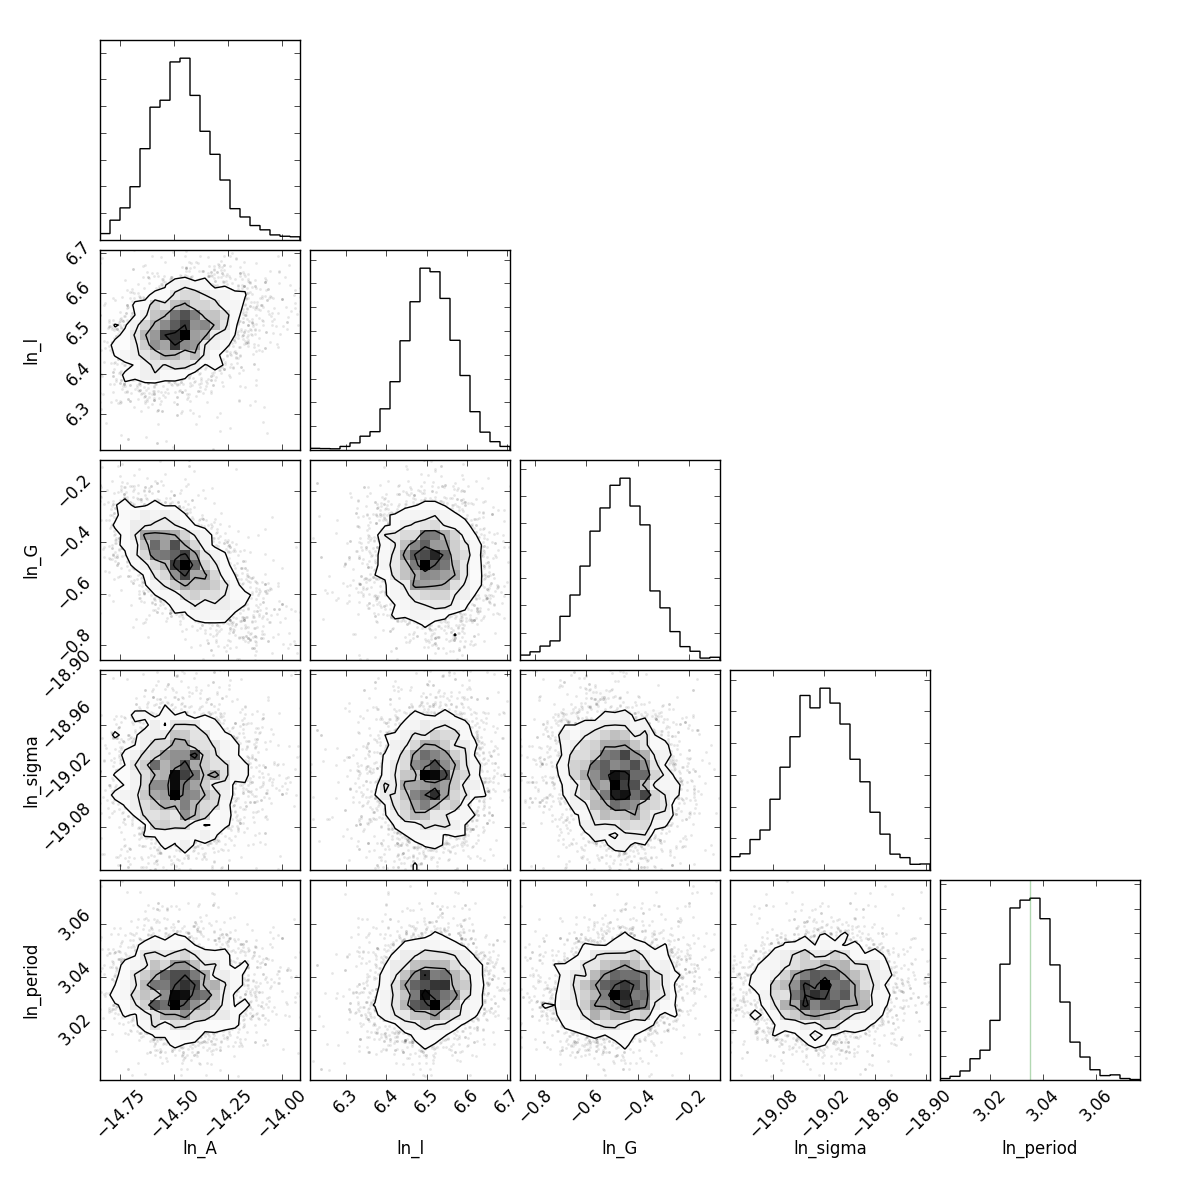
\includegraphics[width=6in, clip=true]{figures/25.png}
\caption{Marginal posterior PDFs of the QP GP model parameters, fit to the
    light curve in figure \ref{fig:demo_lc}.
$\sigma$ is an
additional white noise term added to the diagonal elements of the covariance
matrix. It is the fraction by which the observational uncertainties have been
underestimated. If the uncertainties reported on the data are too small, this
parameter will be non-zero.
    The green line in the period panel shows the injected period.}
\label{fig:gp_posteriors}
\end{center}
\end{figure*}

\section{Real \kepler\ data}
\label{sec:kepler}

In order to test this rotation period inference method on real data,
we applied it to a set of \nkois\ \Kepler\ Object of Interest (KOI)
host stars, \nkoimcq\ of which had rotation periods previously measured by
the ACF method by \citet{Mcquillan2013}.  We use the pipeline-corrected flux
(\texttt{pdcsap\_flux} column in the \Kepler\ light curve table), median-normalized
and unit-subtracted, and mask out all known transiting planet candidate signals.
As with the simulated light curves, we randomly subsample each
light curve by a factor of 30 and split it into segments of about 300 points
for the purposes of evaluating the likelihood.  We also follow the same MCMC
fitting procedure as with the simulated data, using the ACF-based prior as before.

Initially, we also use the same priors on the hyperparameters for the KOIs
as for the simulated light curves (Table \ref{tab:priors}).
However, we found that $\ln l$ and $\ln \Gamma$ tended toward slightly different
values than the simulations.  We also found that the allowed hyperparameter
range that we used for the simulations was too large for the KOI population,
as maybe $\sim$15\% of the fits tended toward corners in the hyperparameter
space, resulting in poor period measurements.  As a result, after this initial
test, we subsequently adjusted the priors and re-fit all the KOIs.  The final
priors and parameter ranges that we used are in Table \ref{tab:koipriors}.

\begin{table*}
\begin{center}
\caption{Priors and bounds on the natural logarithms of the GP model parameters,
        for \Kepler\ light curves}
\begin{tabular}{lcc}
Parameter & Prior & Bounds\\
    \hline
    $\ln A$ & $\mathcal N(-13, 5.7)$ & (-20, 0) \\
    $\ln l$ & $\mathcal N(5.0, 1.2)$ & (2, 8) \\
    $\ln \Gamma$ & $\mathcal N(1.9, 1.4)$ & (0, 3) \\
    $\ln \sigma$ & $\mathcal N(-17, 5)$ & (-20, 0) \\
    $\ln P $ & Uniform / ACF-based & ($\ln 0.5, \ln 100$) \\
\end{tabular}
\end{center}
\end{table*}
\label{tab:koipriors}

Figure \ref{fig:mcquillan} compares the periods inferred with the GP method to the
ACF-based periods from \citet{Mcquillan2013} for the \nkoimcq\ overlapping KOIs.
This comparison shows generally very good agreement, with only a few exceptions,
demonstrating that this method works not only on simulated data, but also on
real data---with the caveat that for any particular data set, some care is needed
regarding the setting the priors and ranges for the GP hyperparameters.

\begin{figure}
\begin{center}
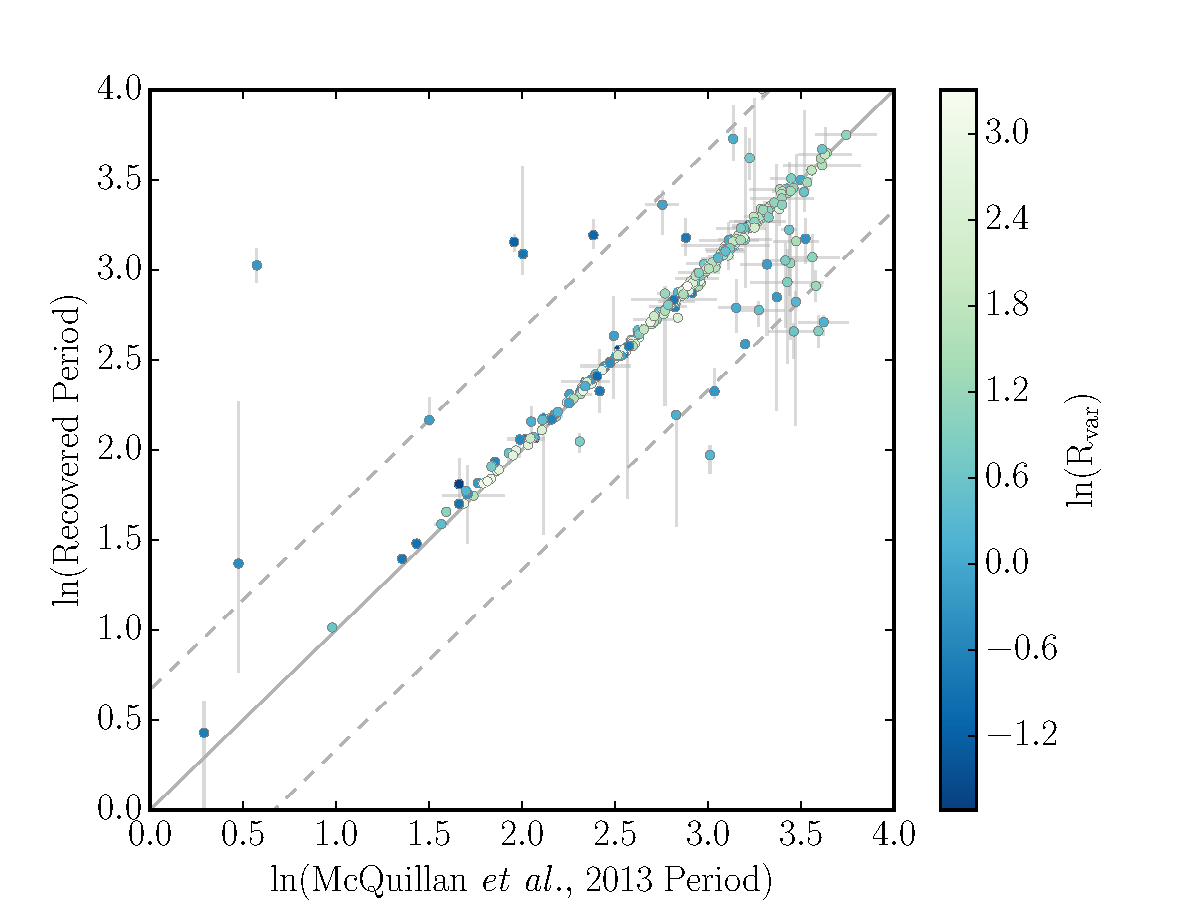
\includegraphics[width=6in, clip=true]{figures/comparison_koi.pdf}
\caption[Comparison with McQuillan results.]
{A comparison of our GP rotation period measurements to those of
\citet{Mcquillan2014}.
The data points are coloured by the range of variability measured by
    \citet{Mcquillan2014}, defined as the interval between the 5th and 95th
    percentiles of normalized flux per period bin in millimagnitudes.
    The results show good agreement.}
\label{fig:mcquillan}
\end{center}
\end{figure}

\section{Discussion}
\label{sec:discussion}

The uncertainties produced by the GP method are more representative than those
produced by the ACF and periodogram methods because the posterior PDF of the
period is explored using MCMC.
Whilst they are an improvement, unfortunately these uncertainties are still
underestimated in the majority cases.
Of the rotation periods recovered from the simulated light curves, only 25\%
of the measured periods lie within 1 $\sigma$ of the true period.
50\% lie within 2 $\sigma$ and 66\% within 3 $\sigma$.
The largest outlier is 114 $\sigma$ away from the true value.
In the majority of these cases the uncertainties are underestimated due to the
multi-modal nature of the period posterior PDFs which makes them difficult to
sample.
The underestimated uncertainties can also be attributed to the model choice.
Although a GP model is more appropriate than a sinusoid, it is still an
imperfect, effective model.
A perfect physical model of the star would produce better results with more
representative uncertainties.

The QP kernel function represents a simplistic effective model of a stellar
light curve.
It adequately describes the data, captures that all-important periodic quality
and is relatively simple, with only a few hyper-parameters.
It also satisfies the requirement to produce positive semi-definite covariance
matrices.
Whilst the QP kernel function evidently captures the periodic qualities of
light curves adequately, it is still a somewhat arbitrary choice.
Another valid choice would be a squared cosine function multiplied by a
squared exponential,
\begin{equation}
k_{i,j} = A \exp \left(-\frac{(x_i - x_j)^2}{2l^2}\right)
\cos\left(\frac{2\pi}{P}\right)
\end{equation}
\label{eq:cos_kernel}
This function produces a positive semi-definite matrix and has the $P$
parameter of interest.
% It may in fact be even {\it more} suited to modelling stellar
% light curves as it describes a Gaussian in frequency space.
% It is easy to imagine a differentially rotating star with a period that is a
% Gaussian in frequency space: the mean frequency would be the frequency at the
% most active latitude, at or near which spots spend the majority of their time
% and the tails would be occupied by spots that drift near the equator or poles.
The main practical difference between this cosine and the QP function is that
the cosine function allows negative covariances and the QP function does not.
Is is realistic to allow negative covariances?
In practice, the ACFs of \Kepler\ light curves often go negative.
However, many stars have two active regions on opposite hemispheres that
produce two brightness dips per rotation.
If the covariance is forced to be negative for two data points that are
separated by half a rotation period, those light curves with two peaks per
rotation period may not be well modelled.
In other words, we do not want to force anti-correlation of points that are
$\frac{1}{2}$ a period apart.
It would be very worthwhile to test this assumption and this alternative
kernel function in future.
If CPU time were not limited there may be some benefit to performing formal
model comparison with different kernel functions.
However, the evidence integral is an ambitious calculation for models with
likelihood functions that take milliseconds to compute, let alone those
involving GPs with light curves containing thousands of data points which can
take minutes.

% Clearly, stellar rotation periods are well represented by the $P$ parameter in
% our QP kernel function, as evidenced by the its impressive ability to recover
% the true rotation periods from the simulated light curves in this work.
% However, it may not be the {\it best} function to use.
% It is, after all, an approximation to the shape of the covariance matrix of a
% real stellar light curve.
% There may be an alternative function which is better suited to capturing
% stellar variability and is able to recover periods even more precisely than
% the QP kernel.
% There may also be an alternative function which is more physically motivated,
% that captures not just the rotation period but also (for example) the spot
% lifetime or differential surface rotation.
% This is beyond the scope of this work but we hope that these questions will be
% answered in the near future.

Not all \kepler\ light curves show evidence of stellar rotation.
In some cases perhaps the star has few or no active regions, it is rotating
pole-on, or it rotates so slowly that the \kepler\ data detrending pipeline
removes any signal.
In other cases there may be another source of variability present in the light
curve, generating a false period detection.
These sources may be physical: \eg\ binary star interactions, intra-pixel
contamination from other astrophysical objects, pulsating variable stars,
asteroseismic oscillations in giants and even stellar activity cycles.
For some of these there is little we can do save attempt to eliminate these
astrophysical false positives via alternative methods, \eg\ apply colour cuts
to avoid giant contamination.
For some however, like the variable stars, they may have distinctive
hyperparameters that identify them, for example long coherence timescales.
Testing this is beyond the scope of this paper but may be an interesting
follow-up study.
As well as astrophysical contamination, there may also be instrumental sources
of contaminating variability: \eg\ temperature variations or pointing shifts
of the \kepler\ spacecraft.
These are unlikely to be periodic and, again, may produce unusual combinations
of hyperparameters.
This is something that we hope to test in future.
In addition to this, there are several other aspects of the GP method we hope
to test in future, listed as follows:.
\begin{itemize}
\item{To perform model selection with different kernel functions. Again, these
tests have not been performed due to the cost of calculating the fully
marginalised likelihood with GPs. This calculation may be prohibitively
expensive, however simpler model selection tests can be performed. For
example, the relative precision of rotation periods recovered using
alternative kernel functions could be tested.}
\item{To design and implement a physically motivated kernel function. We have
only explored the physical interpretation of one parameter in our kernel
function, $P$.
However, the other parameters may also be related to some physical processes.
For example, the overall timescale for covariance fall-off, $l$ may be
related to spot lifetimes.
A star with long spot lifetimes will show little variation in the overall
shape and amplitude of its light curve between rotations and $l$ will be
large.
In contrast, the light curve of a star with short spot lifetimes may display
non-repeating patterns and amplitudes that vary rapidly between rotations.
In this case $l$ will be small.
The $\Gamma$ parameter is related to the number of zero crossings within one
rotation period: when $\Gamma$ is small there are many zero crossings and
vice versa.
Since the number of zero crossings per rotation period is related to the
number of active regions on the surface of the star, this parameter may also
be of physical interest.
In addition, instead of interpreting the parameters of the QP kernel function
used here, it may be possible to design an entirely new kernel function, based
on the physical processes that drive the light curve variability.
This idea is being explored by another member of my research group.}
% \item{To develop a detection criterion to assess whether a rotation period was
% measured.
% Another general problem in rotation period inference is deciding whether a
% real rotation period was measured at all.
% Detection thresholds are usually set using the amplitudes of peaks in LS
% periodograms or ACFs in order to eliminate contaminants.
% Using a GP model it may be possible to do this via model selection: \ie\ are
% the data better described by a periodic model, or a non-periodic model?
% There is more than one way to implement such a model comparison, one way could
% be to use a sum of two kernel functions: one periodic and one non-periodic,
% each with its own amplitude parameter.}
\item{To attempt to detect differential rotation.
We did not test our code on the light curves simulated with differential
rotation in \citet{Aigrain2015} since we were only interested in recovering
the most precise measurements of rotation period possible.
In future we intend to investigate the possibility of recovering
differential rotation by searching for close double peaks in the posterior
PDFs of stars' rotation periods.}
\item{To build in a noise model for \kepler\ data.
Another huge advantage of the GP method is, because it is a {\it generative}
model of the data, the rotation period signal can be modelled at the same time
as systematic noise features.
One can then marginalise over the parameters of the noise model.
This approach would be extremely advantageous for \kepler\ data since
long-term trends are often removed by the \kepler\ detrending pipeline.
Marginalising over the noise model at the same time as inferring the
parameters of interest will insure that the periodic signal is preserved.}
\end{itemize}

\section{Conclusion}

We used the \naigrain\ simulated \kepler-like light curves for solid-body
rotation from \citet{Aigrain2015} and attempted to recover the rotation
periods used to generate them.
Three methods were compared: a Lomb-Scargle periodogram method, an
autocorrelation function method and a new Gaussian process method.
We demonstrate that the GP method produced the most precise and accurate
rotation periods of the three techniques.
As expected, it provides a large improvement over the periodogram method and a
moderate one over the ACF method.
We find that the ACF method often slightly under-predicts the rotation period
due to a subtlety in the standard peak detection algorithm.
% The periodogram method performs poorly because a sinusoid is not a perfect
% model choice for stellar light curves --- they do not always display
% sinusoidal behaviour.
% On the other hand, the ACF method does not rely on any model choice and
In addition, we compared the rotation periods of \kepler\ objects of
interest measured using the GP method to those measured previously by
\citet{Mcquillan2014}.
The good agreement between the two sets of results demonstrates that the GP
method works well on real \kepler\ data.

The GP method provides approximate uncertainties because it produces posterior
PDF samples but they are still imperfect estimates of the intrinsic
uncertainties.
This is because the posterior PDF of the rotation period parameter is, in many
cases, multi-modal.
If it were possible to run an MCMC sampler for an infinite number of steps,
the entire posterior PDF would eventually be sampled, producing an accurate
uncertainty measurement.
We find that only a quarter of the reported uncertainties are representative.

The main aim of this work was to develop a rotation period inference method
that is probabilistic.
Probabilistic periods methods are necessary for hierarchical Bayesian
inference and for performing population analysis.
Using this method to generate a catalogue of probabilistic rotation periods
could, for example, reveal the period distribution of (and therefore
potentially the age distribution) of stars in the Milky Way.
There is still some work to be done on the development of this model such that
the uncertainty estimates are truly representative, but this new method
provides a improvement upon previous methods in that regard.

% acknowledgements
This research was funded by the Simons Foundation and the Leverhulme Trust.
Some of the data presented in this paper were obtained from the Mikulski
Archive for Space Telescopes (MAST).
STScI is operated by the Association of Universities for Research in
Astronomy, Inc., under NASA contract NAS5-26555.
Support for MAST for non-HST data is provided by the NASA Office of Space
Science via grant NNX09AF08G and by other grants and contracts.
This paper includes data collected by the Kepler mission. Funding for the
Kepler mission is provided by the NASA Science Mission directorate.

\appendix

\section{An ACF-informed Prior for Rotation Period}

The autocorrelation function (ACF) has proven to be very useful
for measuring the rotation periods of stars from time-series
photometry.
However, as discussed in the body of this paper, the
ACF-based method has several shortcomings,
most notably the inability to deliver uncertainties, but also
the necessity of several heuristic choices,
such as a timescale on which to smooth the ACF,
how to define a peak, whether the first or second peak
gets selected, and what constitutes a secure detection.
While this paper presents a new MCMC-based method
that avoids these shortcomings,
it seems prudent to still use information available from the ACF.
This Appendix describes how we use the ACF to define a prior on period.

Our strategy here is not to attempt to decide which single
peak in the ACF best represents the true rotation period,
but rather to identify several \emph{candidate} periods and define
a weighting scheme in order to create a non-commital, though useful,
multimodal prior.  While this procedure does not avoid heuristic choices,
the fact that its goal is simply to create a \emph{prior} for a
probabilitistically justified inference scheme rather than
to identify a single correct period softens the potential impact
of these choices.

As another innovation beyond what ACF methods in the literature have
presented, we also bandpass filter the light curves (using a 5th order
Butterworth filter, as implemented in \texttt{SciPy}) before calculating the
autocorrelation.  This suppresses power on timescales shorter than a chosen
minimum period $P_{\rm min}$ and longer than a chosen maximum $P_{\rm max}$,
producing a cleaner autocorrelation signal than an unfiltered light curve.

We use the following procedure to construct a prior for rotation period
given a light curve:
\begin{enumerate}
\item{For each value of $P_i$, where $i = \{1, 3, 5, 10, 30, 50, 100\}$\,d,
we apply a bandpass filter to the light curve using $P_{\rm min}=0.1$\,d
and $P_{\rm max} = P_i$.  We then calculate the ACF of the filtered
light curve out to a maximum lag of $2P_i$ and smooth it with a boxcar
filter of width $P_i/10$.}

\item{We identify the time lag corresponding to the
first peak of each of these ACFs, as well as the first peak's
trough-to-peak height, creating a set of candidate periods
$T_i$ and heights $h_i$.}

\item{We assign a quality metric $Q_i$ to each of these candidate
periods, as follows.  First, we model the ACF as a
damped oscillator with fixed period $T_i$:
\begin{equation}
y = A e^{-t/\tau} \cos{\frac{2\pi t}{T_i} },
\end{equation}
where and $t$ is the lag time,
and find the best-fitting parameters $A_i$ and $\tau_i$ by a non-linear
least squares minimization procedure.  We then define the
following heuristic quality metric:
\begin{equation}
\label{eq:quality}
Q_i = \left(\frac{\tau_i}{T_i}\right) \left(\frac{N_i h_i}{R_i}\right),
\end{equation}
where $h_i$ is the height of the ACF peak at $T_i$,
$N_i$ is the length of the lag vector in the ACF (directly proportional
to the maximum allowed period $P_i$),
and $R_i$ is the sum of squared residuals between the
damped oscillator model and the actual ACF data.  The idea behind this
quality metric to give a candidate period a higher score if

    \begin{enumerate}[(a)]

    \item{it has many regular sinusoidal peaks, such that the decay
        time $\tau_i$ is long compared to the oscillation period $T_i$,}
    \item{the ACF peak height is high, and}
    \item{the damped oscillator model is a good fit (in a $\chi^2$
      sense) to the ACF, with extra bonus for being
      a good fit over more points (larger $N_i$, or longer $P_i$).}

    \end{enumerate}
}

\item{Given this set of candidate periods $T_i$ and quality metrics $Q_i$,
we finally construct a multimodal prior on the $P$ parameter of the GP
model as a weighted mixture of Gaussians:
\begin{equation}
\label{eq:mixture}
p(\ln P) = \frac {\displaystyle \sum_i Q_i \left(0.9\mathcal N(\ln T_i, 0.2) +
                                          0.05\mathcal N(\ln (T_i/2), 0.2) +
                                          0.05\mathcal N(\ln (2 T_i), 0.2) \right)}
                {\sum_i Q_i}.
\end{equation}
That is, in addition to taking the candidate periods themselves as mixture
components, we also mix in twice and half each candidate period at a lower level,
which compensates for the possibility that the first peak in the ACF may actually
represent half or twice the actual rotation period.  The period width of 0.2 in
log space (corresponding to roughly 20\% uncertainty) is again a heuristic choice,
balancing a healthy specificity with the desire to not have the results of
the inference overly determined by the ACF prior.
}

Incidentally, while we use the procedure described here to create a prior on
$P$ which we use while inferring the parameters of the quasi-periodic GP model,
this same procedure may also be used in the service of a
rotation-period estimating procedure all on its own, perhaps being even more
robust and accurate than the traditional ACF method.  We leave exploration of
this possibility to future work.

\end{enumerate}




\bibliographystyle{plainnat}
\bibliography{GProtation}
\end{document}
